\section{Мадэліраванне прататыпа размеркавання патокаў трафіка ў сетках SDN}

У дадзеным раздзеле разглядаецца мадэль невялікай гібрыднай SDN сеткі, якая працуе
пад кантролем вышэапісаннага алгарытму разліку нагрузкі.

Для сімуляцыі сеткі выкарыстоўваецца GNS3 праграма.
GNS3 --- гэта графічны сімулятар сеткі, які дазваляе змадэліраваць віртуальную
сетку з маршрутызатараў і віртуальных машын.

\subsection{Мадэль віртуальнай сеткі}

На малюнку \ref{img: model} прадстаўлена мадэль віртуальнай сеткі з 3 маршрутызатараў і 1 кантролера.

\begin{figure}[h!]
    \centering
    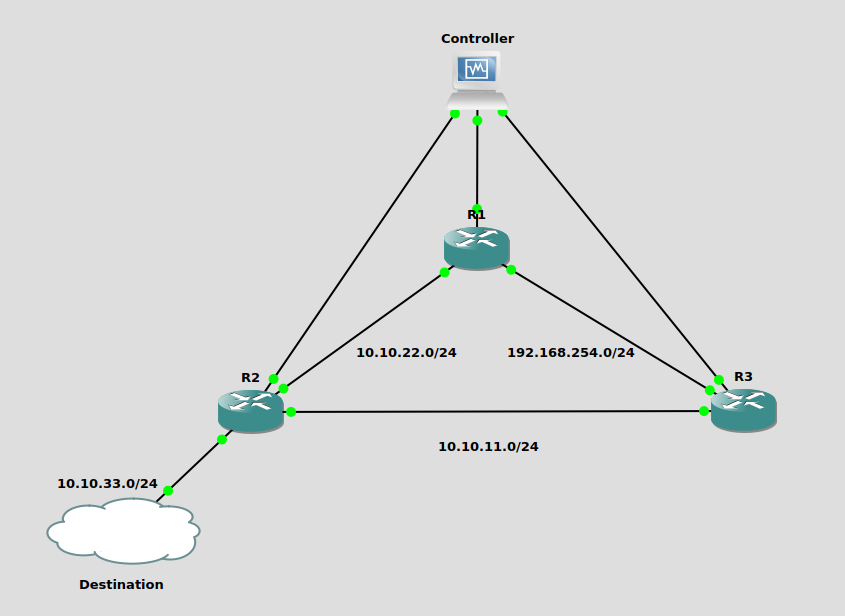
\includegraphics[width=\textwidth]{model.png}
    \caption{Мадэль віртуальнай сеткі}
    \label{img: model} 
\end{figure}

З малюнка \ref{img: model} бачым, што маршрутызатар R1 падключаны да сеткі 10.10.22.0/24 і сеткі 192.168.254.0/24;
маршрутызатар R2 падключаны да сетак 10.10.22.0/24, 10.10.11.0/24 і сеткі 10.10.33.0/24 (прадстаўленая ў відзе loopback інтэрфейса);
маршрутызатар R3 падключаны да 10.10.11.0/24 і 192.168.254.0/24.

Знешні кантролер падключаны да кожнага маршрутызатара. Неабходна заўважыць, што кантролер можа падключацца да маршрутызатараў
як напрамую (як праўдстаўлена на малюнку \ref{img: model}), так і праз іншыя маршрутызатары.

У якасці маршрутызатараў выкарыстоўваюцца маршрутызатары мадэлі CSR1000v (Cisco Cloud Services Router 1000V Series)
з наступнымі параметрамі:
\begin{enumerate}
    \item пратакол маршрутызацыі EIGRP;
    \item прапускная здольнасць на інтэрфейсе ў памеры 10 Кбіт/с;
    \item каэфіцыенты EIGRP метрыкі: $K1 = 1$, $K2 = 1$, $K3 = 1$, $K4 = 0$, $K5 = 0$.
\end{enumerate}

У якасці кантролера выкарыстоўваецца камп'ютар з аперацыйнай сістэмай Debian, на якім
запушчана праграма маніторынгу і пераразліку метрыкі.

\subsection{Першапачатковыя параметры маршрутызатараў}

У дадзеным падраздзеле паказаны пачатковыя параметры на маршрутызатарах (інтэрфейсы, табліца EIGRP маршрутаў, EIGRP тапалогія)
перад падачай трафіка ў сетку.

\subsubsection{Маршрутызатар R1.}

У лістынгу \ref{lst: R1 before/interfaces} прадстаўлена кароткае апісанне ўключаных інтэрфейсаў на маршрутызатары R1.

\lstinputlisting[caption={Уключаныя інтэрфейсы на маршрутызатары R1},%
                            label={lst: R1 before/interfaces},%
                            language=bash]{R1/before/interfaces.txt}

У лістынгу \ref{lst: R1 before/routes} прадстаўлены ўсе даступныя EIGRP маршруты на маршрутызатары R1.


\lstinputlisting[caption={EIGRP маршруты на маршрутызатары R1},%
                            label={lst: R1 before/routes},%
                            language=bash]{R1/before/routes.txt}

З лістынга \ref{lst: R1 before/routes} бачым, што маршрутызатар R1
вывучыў 2 EIGRP маршруты ад суседзяў.
Так для сеткі 10.10.11.0/24 маршрутызатар R1 мае 2 маршруты (балансіроўка
маршрутаў, так як іх метрыкі супадаюць)
праз маршрутызатар R2 (10.10.22.22) і маршртузатар R3 (via 192.168.254.2),
а для сеткі 10.10.33.0/24 мае 1 маршрут праз маршрутызатар R2 (via 10.10.22.22).

У лістынгу \ref{lst: R1 before/topology} прадстаўлена EIGRP тапалогія сеткі на
маршрутызатары R1.

\lstinputlisting[caption={EIGRP тапалогія сеткі на маршрутызатары R1},%
                            label={lst: R1 before/topology},%
                            language=bash]{R1/before/topology.txt}

У EIGRP тапалогіі сеткі можна ўбачыць для кожнай EIGRP сеткі бягучага
Successor-а (маршрутызатар з меншым значэннем FD), а таксама запаснога
Successor-а пры яго наяўнасці.

Напрыклад, для маршрутызатара R1 для сеткі 10.10.11.0/24 існуе 2 Successor-а,
што стала падставайдля ўзнікнення балансіроўкі для дадзенага маршруту
(лістынг \ref{lst: R1 before/routes}).
У той жа час для 10.10.33.0/24 даступны толькі 1 Successor, хаця дадзеная
сетка можа быць дасягнута праз 2 маршрутызатары (via 10.10.22.22 і via 192.168.254.2).


\subsubsection{Маршрутызатар R2.}

У лістынгу \ref{lst: R2 before/interfaces} прадстаўлена кароткае апісанне ўключаных інтэрфейсаў на маршрутызатары R2.

\lstinputlisting[caption={Уключаныя інтэрфейсы на маршрутызатары R2},%
                            label={lst: R2 before/interfaces},%
                            language=bash]{R2/before/interfaces.txt}

У лістынгу \ref{lst: R2 before/routes} прадстаўлены ўсе даступныя EIGRP маршруты на маршрутызатары R2.


\lstinputlisting[caption={EIGRP маршруты на маршрутызатары R2},%
                            label={lst: R2 before/routes},%
                            language=bash]{R2/before/routes.txt}

Можам бачыць, што дадзены маршрутызатар атрымаў 2 EIGRP маршруты ад суседзяў: у сетку 172.31.1.0/24 і 192.168.254.0/24.

У лістынгу \ref{lst: R2 before/topology} прадстаўлена EIGRP тапалогія сеткі на маршрутызатары R2.

\lstinputlisting[caption={EIGRP тапалогія сеткі на маршрутызатары R2},%
                            label={lst: R2 before/topology},%
                            language=bash]{R2/before/topology.txt}

\subsubsection{Маршрутызатар R3.}

У лістынгу \ref{lst: R3 before/interfaces} прадстаўлена кароткае апісанне ўключаных інтэрфейсаў на маршрутызатары R3.

\lstinputlisting[caption={Уключаныя інтэрфейсы на маршрутызатары R3},%
                            label={lst: R3 before/interfaces},%
                            language=bash]{R3/before/interfaces.txt}

У лістынгу \ref{lst: R3 before/routes} прадстаўлены ўсе даступныя EIGRP маршруты на маршрутызатары R3.

\lstinputlisting[caption={EIGRP маршруты на маршрутызатары R3},%
                            label={lst: R3 before/routes},%
                            language=bash]{R3/before/routes.txt}

У лістынгу \ref{lst: R3 before/topology} прадстаўлена EIGRP тапалогія сеткі на маршрутызатары R3.

\lstinputlisting[caption={EIGRP тапалогія сеткі на маршрутызатары R3},%
                            label={lst: R3 before/topology},%
                            language=bash]{R3/before/topology.txt}

\subsection{Работа алгарытму пры перадачы трафіка}

У дадзеным раздзеле разгледзім работу алгарытму на маршрутызатары R1 пры
перадачы трафіка ў сетку.

Для імітацыі перадачы інфармацыі ў сетцы выкарыстоўваўся метад flood ping,
які дазваляе бесперапынку пасылаць вялікія ICMP пакеты ў сетку.

У лістынгу \ref{lst: flood ping} прадстаўлена каманда, якая пачынае 
бесперапынна перадаваць ICMP пакеты памерам 56500 байт у сетку 10.10.33.0/24.

\lstinputlisting[caption={Каманда для імітацыі перадачы трафіка ў сетку},%
                            label={lst: flood ping},%
                            language=bash]{flood_ping.txt}

Як бачна з лістынгу \ref{lst: recalculation} праграма маніторынгу і пераразліку суправаджаецца пастаянным
запісам логаў: пры знаходжанні інтэрфейса, на якім новае значэнне нагрузкі перавышае ўстаноўлены парог,
у логі запісваецца, на якім маршрутызатары адбываецца пераразлік метрыкі, калі значэнне нагрузкі менш за парог,
то ў лог запісваецца старое і новае значэнне нагрузкі на дадзеным інтэрфейсе.

У лістынгу \ref{lst: program output} прадстаўлены лог праграмы да першага пераліку метрыкі для маршрутызатара R1.

\lstinputlisting[caption={Лог праграмы алгарытму для маршрутызатара R1},%
                            label={lst: program output},%
                            language=bash]{program_output.txt}
